\section{Git \& Github}
\begin{frame}
	\frametitle{}
	\tableofcontents[currentsection]
\end{frame}

\subsection{Git}
\begin{frame}
	\frametitle{Git --- Dummkopf \hfill{} LuXeria}
	\framesubtitle{Was ist Git?}
	\begin{columns}
		\begin{column}{5cm}
			\begin{figure}
				
\includegraphics[width=0.8\columnwidth]{git_logo.pdf}
				\caption{neues Git-Logo}
			\end{figure}
			\footnotesize{
			\textbf{git}[\textipa{git}] - a bastard or fool
			\epigraph{ I'm an egoistical bastard, and I name all my projects after myself.
				First Linux, now git.}{Linus Torvalds}
			}\normalsize
		\end{column}
		\begin{column}{5cm}
			\begin{block}{Überblick}
				\begin{itemize}
					\item Verwaltungssystem
					\item nicht linear
					\item dezentral
					\item sicher \& stabil
					\item OpenSource
					\item Plattformunabhängig
				\end{itemize}
			\end{block}
		\end{column}
	\end{columns}
\end{frame}

\begin{frame}
	\frametitle{Git --- nicht linear?\hfill{} LuXeria}
	\framesubtitle{Arbeiten mit Forks und Branches}
	\begin{columns}
		\begin{column}{5cm}
			\begin{figure}
				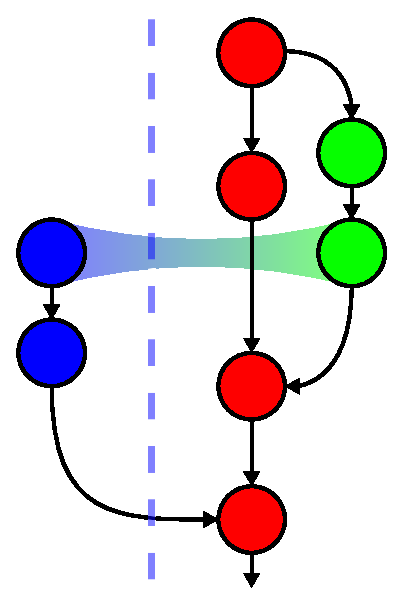
\includegraphics[scale=0.5]{git_tree.eps}\\
				\textcolor{blue}{Fork} -- \textcolor{red}{master} -- \textcolor{darkgreen}{branch}
				\caption{Projetkbaum}
			\end{figure}
		\end{column}
		\begin{column}{5cm}
			\begin{block}{Fork, Master \& Branch}
				\begin{itemize}
					\item \textcolor{red}{Arbeiten am Skript}
					\item \textcolor{darkgreen}{Version HS12}
					\item \textcolor{darkgreen}{Korrekturen im HS12}
					\item \textcolor{blue}{Studenten übernehmen Kopie und erweitern}
					\item \textcolor{red}{Das Beste kommt zusammen für FS13}
				\end{itemize}
			\end{block}
		\end{column}
	\end{columns}
\end{frame}

\begin{frame}
	\frametitle{Git --- dezentral \hfill{} LuXeria}
	\framesubtitle{Offline? Interessiert mich nicht!}
	\begin{columns}
		\begin{column}{5cm}
		\end{column}
		\begin{column}{5cm}
		\end{column}
	\end{columns}
\end{frame}
